\chapter{Presentazione Virtual Machines}
Prima ancora di iniziare a progettare la kill chain da seguire, bisogna rappresentare ed implementare il sistema target di questa esercitazione, su cui andranno realizzate le varie fasi dell'infiltrazione.\\
Partendo dal sistema operativo, la scelta ricade sicuramente su quello maggiormente diffuso ed utilizzato da parte degli utenti ed organizzazioni. Secondo i dati raccolti da StatCounter, Microsoft Windows vede una predominanza assoluta nel panorama degli OS sia aziendali sia personali; sebbene nel 2024 sia aumentato il numero di persone che hanno adottato la versione 11 uscita quattro anni fa, Windows 10 mantiene ancora il primato tra le edizioni in fatto di familiarità, standardizzazione aziendale e compatibilità con le applicazioni. Per quest'ultimo motivo, la maggior parte delle corporazioni adottano un approccio conservativo riguardo la propria infrastruttura, motivato anche dal rischio di un basso livello di compatibilità tra il sistema operativo e le proprie apparecchiature.\cite{os_usage}\\
Sicuramente il 2025 sarà un anno di grande cambiamento per le varie aziende vista la fine del supporto per Windows 10 ad ottobre di quest'anno; questo significa niente più patch di sicurezza o aggiornamenti di drivers, il che porterà a un'esposizione pericolosa dei dati nei sistemi ad eventuali nuovi \textit{threats} che si potranno materializzare dopo quella data. La richiesta di hardware più "potenti", in grado di sostenere le tecnologie di sicurezza implementate nella versione 11, mette in difficoltà non solo gli utenti ma soprattutto diverse organizzazioni, per i motivi sopra riportati.
\begin{figure}[h!]
    \centering
    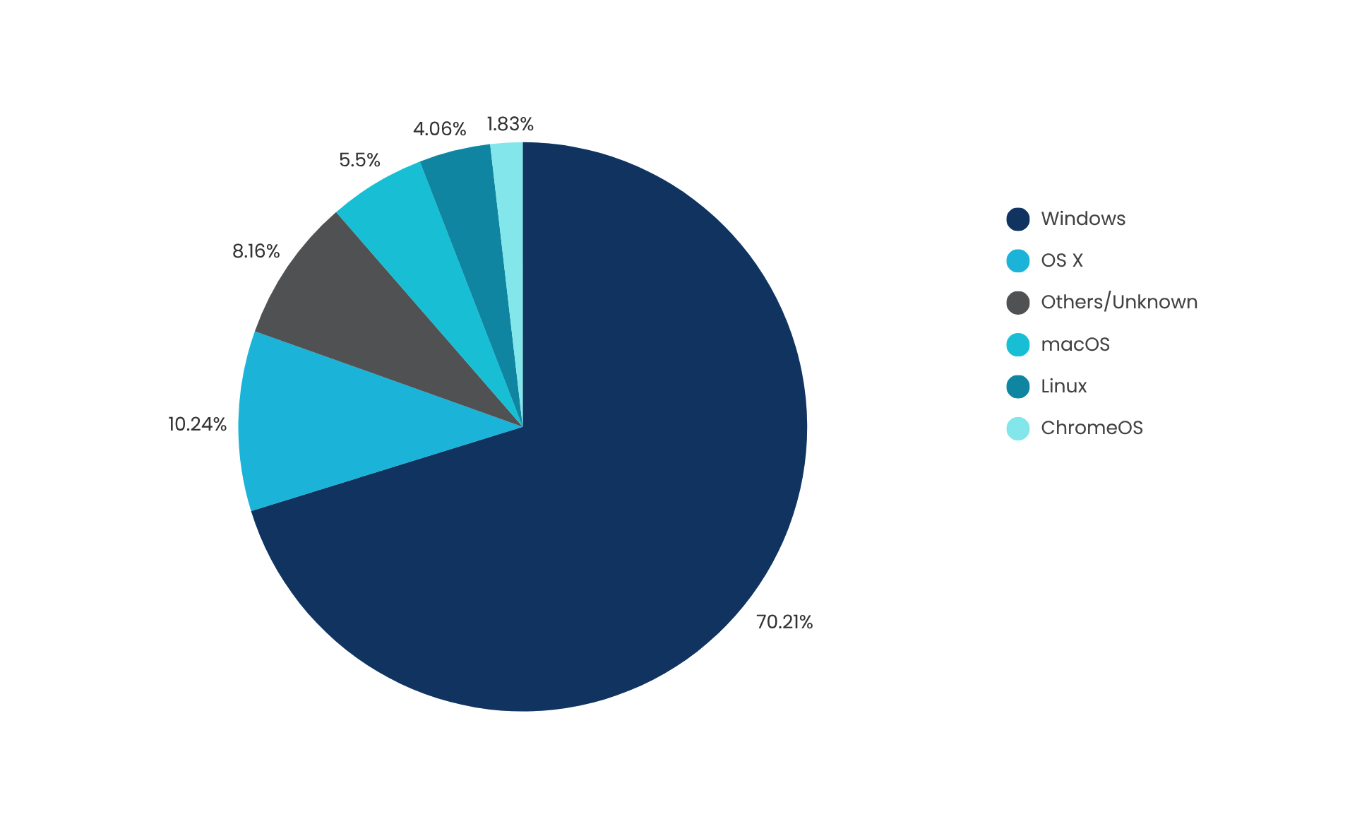
\includegraphics[width=0.75\linewidth]{images/OS_usage.png}
    \caption{Utilizzo OS desktop - Maggio 2025}
\end{figure}
\newpage
\noindent
\begin{figure}[t]
    \centering
    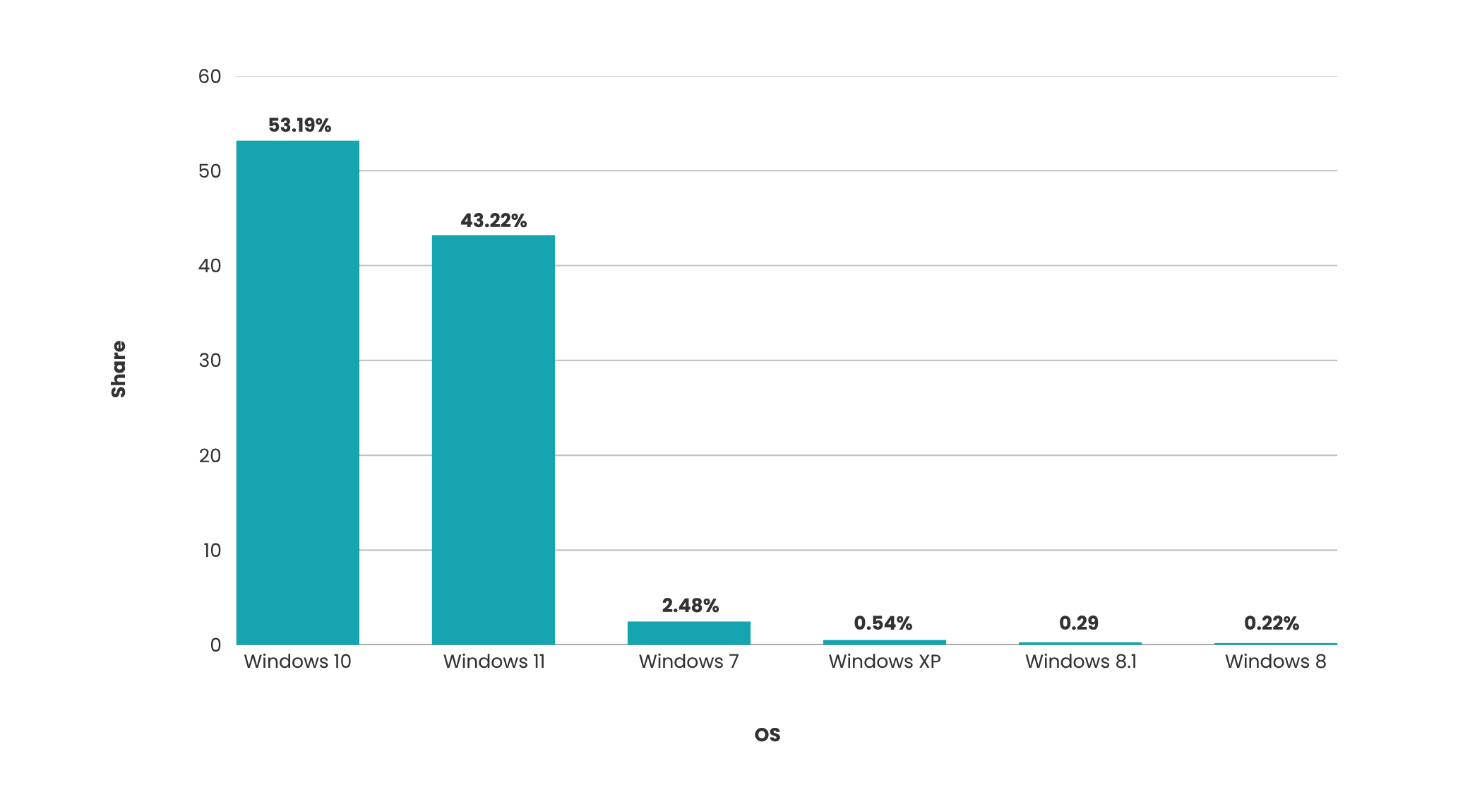
\includegraphics[width=0.75\linewidth]{images/Windows_usage.png}
    \caption{Utilizzo OS Windows - Maggio 2025}
\end{figure}
È intuitivo comprendere le motivazioni che hanno portato alla scelta del sistema operativo per la macchina; considerando la necessità di comprare componenti hardware nuovi e gli eventuali costi, si prospetta un 2026 con una grande disponibilità di infrastrutture obsolete vista l'incompatibilità dell'hardware con Windows 11, come descritto precedentemente.\\
Entrambe le macchine virtuali sono state realizzate tramite il software Oracle VirtualBox.\textsuperscript{TM}

\section{Windows VM\label{win}}
Presi in considerazione i vari dati estratti dalle analisi di mercato e dalla maggior parte degli utenti, nella macchina target è stato installato Windows 10 Pro con alcune configurazioni in più programmate in modo da rendere lo scenario abbastanza realistico.

    \subsection{Firewall}
    Rappresenta una delle numerose linee di difesa all'interno di un'organizzazione. In particolare, gestiscono il transito dell'attività web consentita e vietata all'interno di una rete privata, documentando il tutto tramite dei log di audit per fare riferimento a quanto è stato consentito o bloccato. Nel firewall della macchina virtuale sono state aggiunte delle regole in modo che l'host rispecchi un panorama possibile di sistema all'interno di un'infrastruttura privata. Di seguito la lista dei comandi eseguiti su Powershell per l'inserimento delle nuove connessioni consentite:\\

    \noindent
    \textsf{Connessioni HTTP dai server dell'enterprise}
    \begin{Verbatim}
    New-NetFirewallRule -DisplayName "HTTP_Proxy"
    -Direction Inbound -Action Allow -Protocol TCP -LocalPort 80
    -RemoteAddress *IP server organizzazione* -Profile Domain,Private
    \end{Verbatim}

    \noindent
    \textsf{Connessioni HTTPS da proxy server}
    \begin{Verbatim}
    New-NetFirewallRule -DisplayName "HTTPS_Proxy"
    -Direction Inbound -Action Allow -Protocol TCP -LocalPort 443
    -RemoteAddress *IP server organizzazione* -Profile Domain,Private
    \end{Verbatim}

    \noindent
    \textsf{MSSQL dal livello applicazione della subnet}
    \begin{Verbatim}
    New-NetFirewallRule -DisplayName "MSSQL_AppTier"
    -Direction Inbound -Action Allow -Protocol TCP -LocalPort 1433
    -RemoteAddress *Subnet organizzazione* -Profile Domain,Private
    \end{Verbatim}

    \noindent
    \textsf{Ping solo da host monitorato}
    \begin{Verbatim}
    New-NetFirewallRule -DisplayName "ICMP_Monitor"
    -Direction Inbound -Action Allow -Protocol ICMPv4
    -IcmpType 8 -RemoteAddress *IP host sicuro* 
    -Profile Domain,Private      
    \end{Verbatim}

    L'insieme di queste regole è volutamente "semplice" essendo il focus del progetto più concentrato su Caldera e sull'emulazione dell'avversario.\\
    
    \subsection{Microsoft SQL Server 2019}
    Secondo dati raccolti semestralmente da SQL ConstantCare\textregistered\cite{mssql} nell'estate 2025, MSSQL 2019 si presenta ancora come un server altamente utilizzato tra le aziende globali, crescendo addirittura di qualche punto percentuale rispetto allo scorso semestre. Quindi, è considerata un'ottima scelta per un ambiente d'esercitazione. Per personalizzarla al meglio, ed essendo dati importanti per il futuro exploit che si andrà ad eseguire, ho creato il database vulnerabile chiamandolo "VulnUserDB" ed è stata creata una tabella \textit{Users} contenente i dati di possibili impiegati registrati all'interno dell'enterprise:
    \begin{enumerate}
        \item \texttt{id}: Codice identificativo di ogni dipendente.
        \item \texttt{username}: Nickname scelto all'interno del server.
        \item \texttt{password}: Chiave di accesso al server (volutamente non crittografato).
    \end{enumerate}
    L'utente target di questo attacco è ovviamente il \texttt{SA} (System Administrator), il quale ha pieno controllo su ogni impostazione del server; in particolare, è capace di cambiare una funzione disponibile all'interno di MSSQL che permette l'abilitazione di un terminale da cui poter avviare comandi Powershell: \texttt{xp\_cmdshell}.\\
    Viene da sé che questa feature rappresenta una risorsa molto pericolosa per chiunque sia in grado di ottenere le credenziali dell'Amministratore e connettersi in remoto: è un punto perfetto da cui iniziare un vettore d'attacco ed è la vulnerabilità utilizzata per piazzare l'agente all'interno della macchina. È possibile ampliare a piacimento non solo gli utenti autorizzati ad accedere al server e le loro autorizzazioni, ma anche creare database nuovi o aggiungere un numero arbitrario di tabelle con relativi dati.\\
    % Scrivi qualcosa in più in modo da riempire la pagina in bianco
    
    \subsection{Applicazione Web}
    \noindent
    \begin{figure}[H]
        \centering
        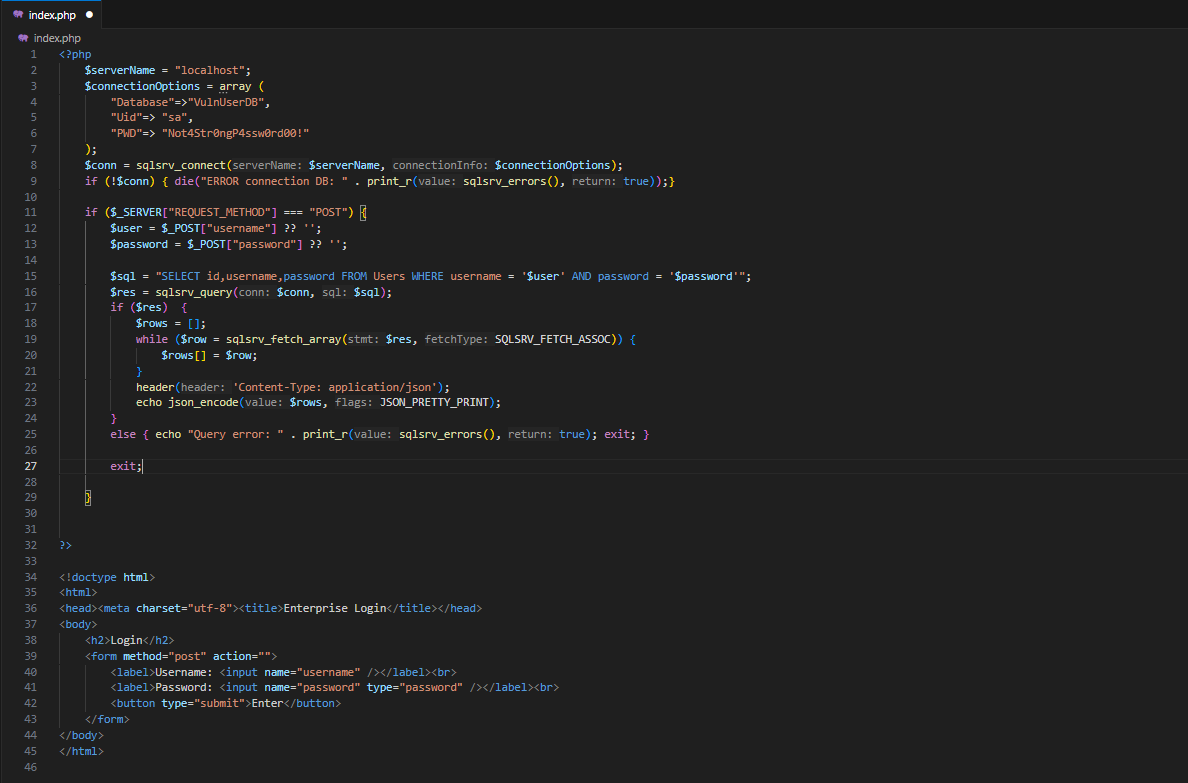
\includegraphics[width=\textwidth]{images/web.png}
        \caption{Source code dell'applicazione web}
    \end{figure}
    Siccome la progettazione di una complessa applicazione web va al di fuori dell'ambito di questo tirocinio, è stato fatto uso di un software molto usato ancora oggi che permette la creazione e l'avvio di server web anche in locale, ossia \textsc{XAMPP}.\\
    Facendo uso dei linguaggi \textsc{PHP} ed \textsc{HTML} è stata creata una semplice pagina web da cui è possibile effettuare il login utilizzando le credenziali conservate nella tabella \textit{Users} sopra citata. Nella pagina successiva, a seconda del risultato del controllo sulla corrispondenza delle credenziali presentate, ho fatto in modo di restituire, in formato \texttt{.json}, i dati collezionati dalla query (risultano vuoti nel caso in cui essa sia vuota).
    Come si può notare dal codice sorgente, un exploit che salta subito all'occhio è la gestione della query da passare al server in cui è possibile bypassare il controllo della password o, addirittura, farsi restituire i dati salvati nel database attraverso la tecnica dell'SQL Injection sul database presente.\\[1.5em]

    \noindent
    {\bfseries\Large{SQL Injection}}\\[1em]
    Si può situare la nascita di questa vulnerabilità contemporanea all'inizio degli sviluppi di database relazionali, quindi nel lontano 1998. La maggior parte dei furti di dati è avvenuto principalmente a causa di questo tipo di exploit ed ancora oggi molte aziende non sono in grado di mitigarlo completamente.\\
    Per definizione, l'SQL Injection sfrutta il mancato controllo dell'input ed invia del codice malevolo per manipolare la query richiesta in modo da accedere a dati altrimenti inaccessibili, bypassare l'autenticazione ed entrare all'interno del server senza aver bisogno di fare brute force sulla password o, addirittura, cancellare dei dati presenti nel database. Esistono diversi tipi di SQLi:
    \begin{itemize}
        \item \textbf{Inband:} Il più comune e semplice da implementare, avviene quando l'attaccante è in grado di utilizzare lo stesso canale di comunicazione sia per lanciare l'attacco sia per ricevere i dati ricercati. Tra sottotipi di questo metodo abbiamo anche: error-based e union-based.
        \item \textbf{Blind:} L'attaccante è in grado di ricostruire la struttura del database grazie ai payload inviati ed osservando la risposta dell'applicazione web e il conseguente comportamento del server di database. Come esplicitato dal nome, l'attaccante non è in grado di visualizzare risultati provenienti da un attacco inband. Come sottotipi si hanno: boolean-based e time-based.
        \item \textbf{Out-of-band:} Meno diffusa rispetto altre per via del prerequisito di avere delle determinate funzioni all'interno del DB vittima. È l'opposto dell'SQLi inband e dipende dall'abilità del database di effettuare richieste DNS o HTTP per inviare dati all'attaccante.
    \end{itemize}
    Il primo tipo di SQLi è quello sfruttato in questo laboratorio, i prerequisiti sono stati soddisfatti in modo da rendere possibile l'injection inband.

    
\section{Ubuntu VM}
Per usufruire al meglio degli strumenti utilizzati principalmente dai Red Team durante l'esercitazione, il server Caldera è stato installato all'interno di una VM Ubuntu 25.04, seguendo gli step di configurazione presenti nel sito ufficiale del framework in cui è stato necessario installare componenti aggiuntivi molto semplici grazie all'Advanced Package Tool presente nei sistemi GNU\textbackslash Linux.
\begin{itemize}
    \item \texttt{sudo apt install nodejs}
    \item \texttt{sudo apt install golang}
    \item (Opzionale, ma consigliato) Utilizzare Google Chrome.
\end{itemize}
Inoltre, al fine di racchiudere in un unico contesto le risorse scaricare, è stato creato un ambiente virtuale Python in cui sono stati esportati tutti i file di configurazione di Caldera. Come versione scelta per l'interpretazione dei comandi si è optato per la \texttt{3.10.14} grazie alla risorsa \textsc{pyenv} che permette di installare più versioni di Python nell'host, poiché la più recente potrebbe creare problemi durante l'installazione delle librerie richieste dal framework presenti nel file \texttt{caldera/requirements.txt}.
\begin{Verbatim}[breaklines=true]
    curl https://pyenv.run | bash
\end{Verbatim}
Dopo aver scaricato i file necessari, bisogna aggiungere il path alla configurazione della shell scritta in \texttt{.bashrc} (o \texttt{.zshrc} a seconda della distribuzione).
\begin{Verbatim}
    export PATH="$HOME/.pyenv/bin:$PATH"
    export PYENV_ROOT="$HOME/.pyenv"
    export PATH="$PYENV_ROOT/bin:$PATH"
    eval "$(pyenv init -)"
    eval "$(pyenv virtualenv-init -)"
\end{Verbatim}
\vspace{0.5em}
Una volta installato bisognerà semplicemente riavviare la shell e sarà possibile utilizzare i comandi di \textsc{pyenv}.
\vspace{0.5em}
\begin{Verbatim}
    pyenv install 3.10.14
    pynev global 3.10.14 # Per utilizzare la versione installata
\end{Verbatim}
\vspace{0.5em}
Si proceda al setup dei requisiti in \texttt{caldera/requirements.txt} solo dopo essere certi di star usando la versione di Python adatta (si consiglia la stessa di questo progetto o una precedente alla 3.13)
Ora rimane la questione del come riuscire a comunicare con il server MSSQL attraverso la macchina attaccante, la risposta si trova nel tool ufficiale Microsoft \texttt{sqlcmd} il quale è un validissimo strumento interattivo ed affidabile per quanto riguarda scripting, query ed autenticazione. È possibile scaricarlo tramite terminale nella propria distribuzione Linux Ubuntu attraverso una serie di comandi script (nel sito web ufficiale di Microsoft si fa riferimento solo ad un'installazione per Ubuntu 24.04; tuttavia è compatibile anche con la 25.04 senza nessun errore di dipendenze ma, nel caso si dovessero riscontrare, è consigliabile utilizzare un docker).
Con i privilegi root, si registra e si installa la repository di Microsoft su Ubuntu.
\vspace{0.5em}
\begin{Verbatim}
    curl -sSL -O https://packages.microsoft.com/config/ubuntu/ \
    24.04/packages-microsoft-prod.deb

    sudo dkpg -i package-microsoft-prod.deb
\end{Verbatim}
\vspace{0.5em}
È bene aggiornare la lista di risorse del sistema, dopodiché si esegue il comando per installare il tool grazie all'unixODBC package.
\vspace{0.5em}
\begin{Verbatim}
    sudo apt-get update
    sudo apt-get install mssql-tools18 unixodbc-dev
\end{Verbatim}
\vspace{0.5em}
Nel caso si richieda di aggiornare il tool, basterà lanciare questo semplice script.
\vspace{0.5em}
\begin{Verbatim}
    sudo apt-get update
    sudo apt-get install mssql-tools18
\end{Verbatim}
\vspace{0.5em}
Per verificare la corretta implementazione, effettuiamo un test di connessione in cui accediamo con credenziali precedentemente create nel server e come output dovrebbe uscire qualcosa di simile alla figura sottostante:
\begin{figure}[H]
    \centering
    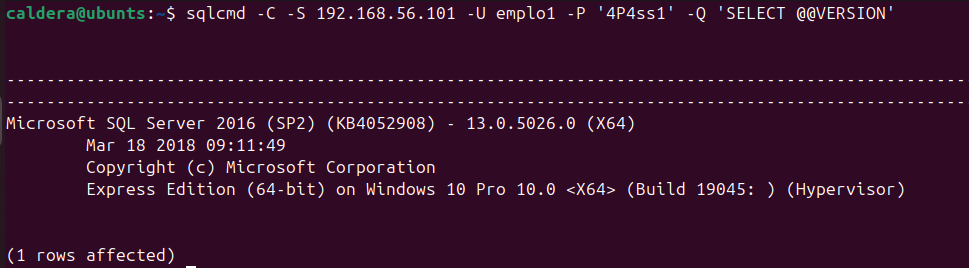
\includegraphics[width=\textwidth,trim= 1 0 0 1,clip]{images/SqlCMD_screen.png}
    \caption{Risultato query su versione database}
\end{figure}
Dopo aver avuto conferma della corretta installazione di \texttt{sqlcmd} siamo pronti ad iniziare il nostro laboratorio sulla macchina Windows.